\documentclass[10pt, conference]{IEEEtran}
% \IEEEoverridecommandlockouts
% The preceding line is only needed to identify funding in the first footnote. If that is unneeded, please comment it out.
%Template version as of 6/27/2024

\usepackage[T1]{fontenc}
\usepackage{cite}
\usepackage{url}
\usepackage{amsmath,amssymb,amsfonts}
\usepackage{algorithmic}
\usepackage{graphicx}
\graphicspath{{./images/}}
\usepackage{textcomp}
\usepackage{xcolor}
\usepackage[UTF8]{ctex}
\usepackage[english]{babel}
\usepackage{microtype}
\usepackage{multirow}
\usepackage{booktabs}   
\usepackage{adjustbox}
\def\BibTeX{{\rm B\kern-.05em{\sc i\kern-.025em b}\kern-.08em
    T\kern-.1667em\lower.7ex\hbox{E}\kern-.125emX}}

\newcommand{\todo}[1]{\textcolor{red}{TODO: #1}}
\begin{document}

\title{V3}

\author{\IEEEauthorblockN{1\textsuperscript{st} Chunyu Yang}
    \IEEEauthorblockA{\textit{School of Computer Science} \\
        \textit{Fudan University}\\
        Shanghai, China \\
        22307140114@m.fudan.edu.cn}
}

\maketitle

\begin{abstract}
    The increase of low Earth orbit (LEO) satellite constellations has intensified interference risks with geostationary (GSO) networks, demanding scalable, real-time detection solutions. Existing deep learning approaches either sacrifice accuracy for efficiency or fail to adapt to dynamic spectral overlaps. We propose DualAttWaveNet, a multimodal autoencoder integrating bidirectional cross-domain attention and multi-scale wavelet regularization to address these challenges. Our framework processes synchronized time-domainand frequency-domain signal, fusing them via a lightweight mutual attention mechanism without computational bottlenecks. Wavelet transform regularization enforce reconstruction fidelity across temporal and spectral resolutions.
\end{abstract}

\begin{IEEEkeywords}
    interference detection, multimodal fusion, bidirectional attention, wavelet transform
\end{IEEEkeywords}

\section{Introduction}

The rapid increase of non-geostationary orbit (NGSO) satellite constellations, fueled by demand for low-latency broadband and advancements in cost-effective launch technologies, has intensified orbital congestion in low-Earth orbit (LEO). With thousands of satellites now competing for limited spectrum resources, the risk of cross-system interference between NGSO and geostationary orbit (GSO) networks has reached critical levels. Spectral overlap between these systems disrupts service reliability, as even minor deviations in orbital positioning or beam alignment can generate harmful interference-to-noise ratios (I/N) \cite{itu2020}. Mitigating these effects requires real-time, adaptive detection mechanisms capable of discerning interference within dynamic, multi-operator environments. However, there has been an absence of scalable solutions for modern satellite coexistence scenarios.

Standardized regulatory frameworks define preventive interference thresholds and aggregation methodologies to limit harm to critical satellite services. The International Telecommunication Union (ITU) mandates a $-10~\text{dB}$ $I / N$ ceiling over 99.9\% of operational intervals to protect GSO receiver integrity \cite{itur2017ProtectionCriteriaOperation}. Central to compliance is the Equivalent Power Flux Density (EPFD) metric, a tool codified in ITU Radio Regulations to address distributed interference risks. By aggregating and bounding the cumulative power flux density from all non-geostationary (NGSO) transmitters, EPFD ensures NGSO systems restrict their aggregate emissions at GSO terminals before operations \cite{itur2002AggregateDownlinkEquivalent}.

Traditional interference detection operates reactively through signal analysis after interference occurs. For example, energy detection (ED) identifies anomalies by summing squared signal amplitudes $E_{n } = \sum y_n[m]^{2}$ over a fixed time window and flagging energy exceeding a predefined threshold \cite{kay2009fundamentals}. While ED is computationally efficient, its static thresholding fails to distinguish weak interference from noise in low-SNR regimes, leading to missed detections  \cite{saifaldawlaGenAIBasedModelsNGSO2024}. Enhanced techniques like cyclostationary feature detection improve robustness by exploiting periodic signal properties \cite{experimentalCyclostationary}, yet they cause significant computational costs when applied to LEO systems. Two-step hybrid approaches integrating pilot cancellation and hardware-based filtering have demonstrated limited success but lack the adaptability to support evolving satellite architectures \cite{wangCoFrequencyInterferenceAnalysis2020}.

Recent advances in machine learning (ML) seek to mitigate the shortcomings of traditional detection frameworks. Initial efforts utilized deep neural networks, such as  LSTM-based architectures \cite{pellacoSpectrumPredictionInterference2019}, to identify interference by processing in-phase/quadrature (IQ) signal components or time-domain amplitude signal. Contemporary methodologies view the detection task as an anomaly discrimination problem, training models to isolate interference from nominal transmissions by learning their intrinsic signatures. Autoencoder-based strategies \cite{saifaldawlaConvolutionalAutoencodersNonGeostationary2024}, for instance, reconstruct idealized interference-free signals from raw inputs; significant energy deviations between the input and reconstructed waveforms are flagged as potential interference. Transformers have further pushed detection boundaries, attaining state-of-the-art area-under-curve (AUC) scores by modeling long-range spectral and temporal correlations in signal \cite{saifaldawlaGenAIBasedModelsNGSO2024}. Nevertheless, these architectures impose substantial computational burdens during training, making them impractical for latency-sensitive satellite operations.

To overcome these barriers, we propose DualAttWaveNet, a multimodal architecture that unifies time-frequency signal representations, achieving an AUC of 0.9327 while reducing GFLOPS to 5.19. The core contributions include:

\begin{enumerate}
    \item Bidirectional Cross-Domain Attention: A lightweight mutual attention mechanism that dynamically fuses temporal waveforms and spectral features, learning interdependencies between domains without concatenation bottlenecks.
    \item Multi-Scale Wavelet Regularization: A loss function enforcing reconstruction fidelity across four predefined wavelet scales, aligning interference patterns with broader spectral trends for robust detection.
    \item Our detector is validated using the system model in \cite{saifaldawlaGenAIBasedModelsNGSO2024}, which synthesizes realistic GSO/LEO coexistence scenarios. This ensures evaluation under interference conditions mirroring actual orbital dynamics and spectral constraints.
\end{enumerate}

\section{System Model}
\label{sec:system_model}

\subsection{Interference Scenario Configuration}
An interference scenario between geostationary orbit (GSO) and low Earth orbit (LEO) satellite systems is considered, as conceptually illustrated in \figurename~\ref{fig:interference-scenario}. The GSO satellite operates as the primary communication node, while multiple LEO satellites from non-geostationary systems introduce unintended interference components observed at a GSO ground station (GGS). The composite received waveform contains both desired carrier signals and interference.

\begin{figure}[tb]
    \centering
    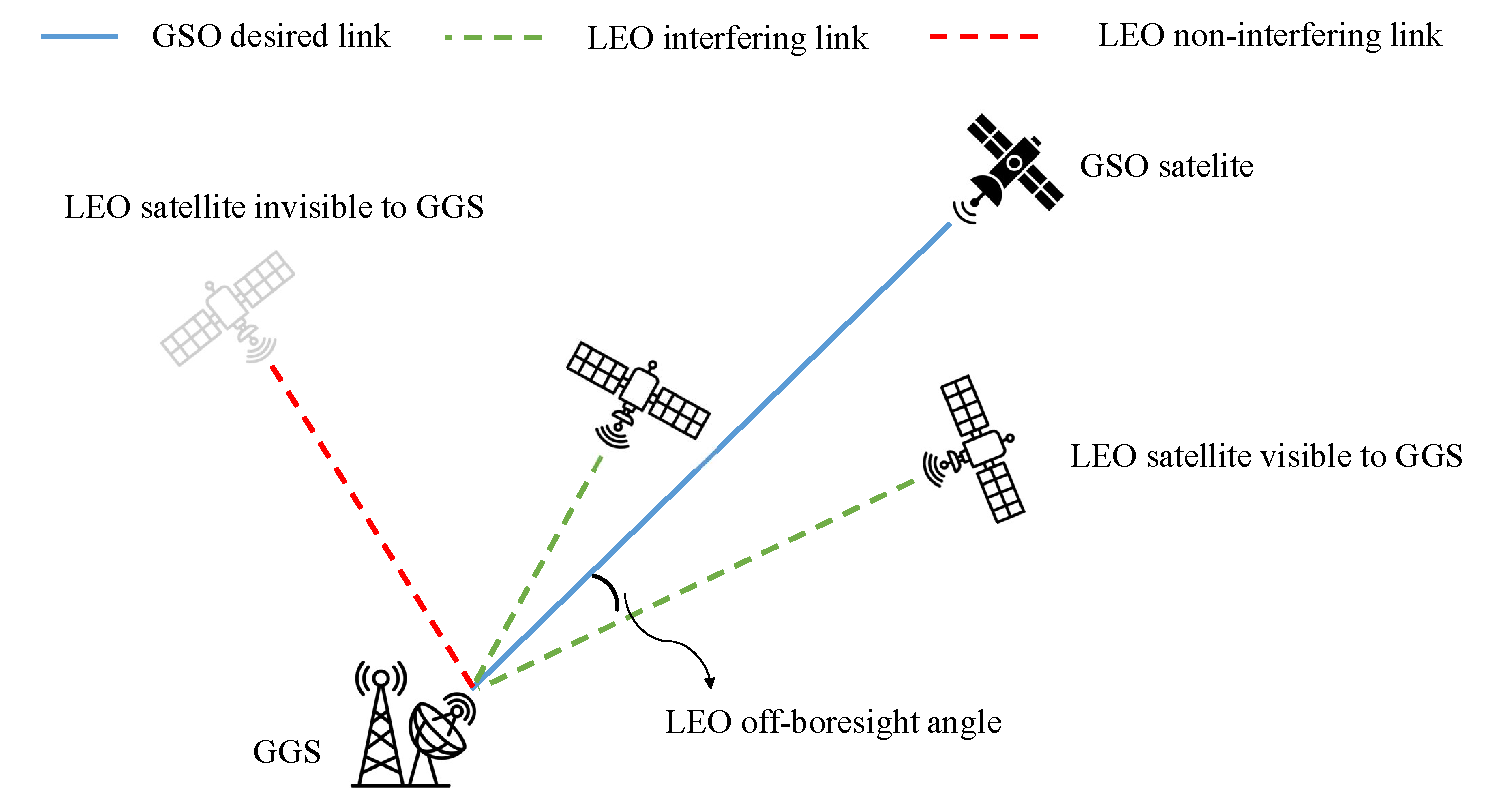
\includegraphics[width=\linewidth]{system-model.pdf}
    \caption{Interference scenario between GSO and LEO satellite systems.}
    \label{fig:interference-scenario}
\end{figure}

\subsection{Link Budget Analysis}
The received GSO carrier power is determined through classical satellite link relationships:

\begin{equation}
    C = \frac{\text{EIRP}_{\text{gso}} \cdot G_{\text{r, gso}}(\theta_0)}{L_{\text{FS, gso}} \cdot L_{\text{add}}}
    \label{eq:carrier_power}
\end{equation}

where $G_{\text{r, gso}}(\theta_0)$ denotes the maximum receive antenna gain at boresight angle $\theta_0$, $L_{\text{FS, gso}}$ represents free-space path loss, and $L_{\text{add}}$ accounts for aggregate atmospheric impairments.

Interference contributions from $K$ LEO satellites are modeled as individual components:

\begin{equation}
    I_k = \frac{\text{EIRP}_k \cdot G_{\text{r, k}}(\theta_k) \cdot B_{\text{adj, k}}}{L_{\text{FS, k}} \cdot L_{\text{add}}}
    \label{eq:interference_power}
\end{equation}

The angular gain term $G_{\text{r, k}}(\theta_k)$ reflects spatial relationships caused by LEO orbital motion, while $B_{\text{adj, k}} \in [0,1]$ is the spectral overlap between GSO and LEO transmissions.

The composite signal quality is characterized through the carrier-to-interference-plus-noise ratio:

\begin{equation}
    \text{CINR} = \frac{C}{\sum_{k=1}^{K}I_k + k_{\text{B}}TB}
    \label{eq:CINR}
\end{equation}

where $k_{\text{B}}$ denotes the Boltzmann constant, $T$ the system noise temperature, and $B$ the operational bandwidth.

\subsection{Signal Composition}
The signal received by physical layer at the GGS has three components:

\begin{align}
    y(t) =\, & x(t)\sqrt{\text{CNR}}\, (\text{Desired GSO}) \nonumber                                                 \\[0.5em]
             & + \sum_{k=1}^{K} i_k(t)e^{j2\pi \Delta f_k t}\sqrt{\text{INR}_k}\, (\text{LEO interference}) \nonumber \\[0.5em]
             & + \zeta(t)\, (\text{Thermal noise})
\end{align}

where $\Delta f_k = f_{\text{c},k} - f_{\text{c,gso}}$ captures carrier frequency offsets from Doppler effects and orbital dynamics. The exponential terms induce time-varying phase rotations proportional to relative satellite motion.

Dual signal representations are derived for machine learning processing:
\begin{itemize}
    \item Time-domain: $y^A$ captures instantaneous amplitude variations through uniform sampling
    \item Frequency-domain: Welch's power spectral density estimation generates logarithmic magnitude spectra via overlapping windowed transforms: $y^F = 10\log_{10}(\phi(y(t)))$
\end{itemize}

\section{Proposed Deep Learning Model}

We propose DualAttWaveNet, an autoencoder that takes both time and frequency domain signal as input, and try to reconstruct both of them. The model consists of separate encoder and decoder for both domains, and a fusion module that utilizes bidirectional attention before concatenating. The loss function is regularized with wavelet transform to enforce reconstruction fidelity across multiple scales.

\subsection{Bidirectional Attention}
\label{subsec:bi_attn}

We propose a parameter-efficient mutual attention mechanism for cross-modal feature fusion. Unlike conventional multi-head attention in \cite{vaswaniAttentionAllYou2017}, our design employs single-head dot-product attention with spatial reduction to minimize computational overhead while maintaining inter-domain alignment capacity, as show in  \figurename~\ref{fig:bidirectional-attention}.

\begin{figure}[tb]
    \centering
    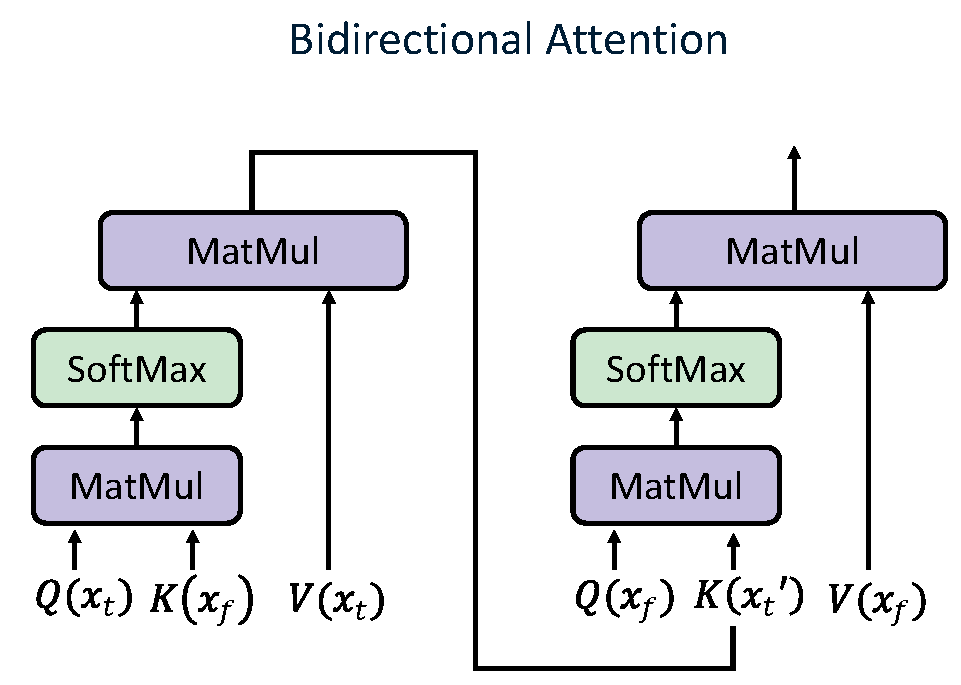
\includegraphics[width=0.9\linewidth]{bidirectional-attention.pdf}
    \caption{DualAttnWaveNet's bidirectional attention mechanism. Both attention phase share the same parameter $Q, K$ and $V$. To decrease channel numbers, they are implemented as 1d-Convolution.}
    \label{fig:bidirectional-attention}
\end{figure}

Given input feature maps $\mathbf{X} \in \mathbb{R}^{B \times C \times L}$ (temporal domain) and $\mathbf{Y} \in \mathbb{R}^{B \times C \times L}$ (spectral domain), the mutual attention operator computes:

\begin{equation}
    \begin{aligned}
        \text{MutualAttn}(\mathbf{X}, \mathbf{Y})    & = \mathbf{X} + \gamma \cdot \text{AttentionGate}(\mathbf{X}, \mathbf{Y})                        \\
        \text{AttentionGate}(\mathbf{X}, \mathbf{Y}) & = \mathbf{V}_y \cdot \text{Softmax}\left(\frac{\mathbf{Q}_x \mathbf{K}_y^\top}{\sqrt{d}}\right)
    \end{aligned}
\end{equation}

where $\gamma$ is a learnable scalar initialized to 0, $\mathbf{Q}_x = \mathcal{W}_Q(\mathbf{X}) \in \mathbb{R}^{B \times L \times \frac{C}{8}}$, $\mathbf{K}_y = \mathcal{W}_K(\mathbf{Y}) \in \mathbb{R}^{B \times \frac{C}{8} \times L}$, and $\mathbf{V}_y = \mathcal{W}_V(\mathbf{Y}) \in \mathbb{R}^{B \times C \times L}$. The projection matrices $\mathcal{W}_{Q,K,V}$ implement 1D convolutions with kernel size 1, reducing channel dimensions by $8\times$ for queries/keys to optimize memory footprint.

The compatibility scores between temporal ($\mathbf{X}$) and spectral ($\mathbf{Y}$) features are computed through matrix multiplication of the reduced-channel representations. This produces an $L \times L$ affinity matrix that represents position-wise cross-domain correlations before applying row-wise softmax normalization.

To preserve original feature stability during early training, the residual connection is initially dampened ($\gamma=0$) and progressively strengthened through learning. The symmetric architecture applies identical attention operations in both temporal→spectral and spectral→temporal directions, in sequential form:

\begin{equation}
    \begin{aligned}
        \mathbf{\widehat{X}} & = \text{MutualAttn}(\mathbf{X}, \mathbf{Y}) \\
        \mathbf{\widehat{Y}} & = \text{MutualAttn}(\mathbf{Y}, \mathbf{X})
    \end{aligned}
\end{equation}

This bidirectional design shares parameters across both call of attention, enables joint refinement of both modalities without major comutational overhead.

\subsection{Wavelet-Domain Spectral Regularization}
\label{subsec:wavelet}

Our temporal-spectral analysis employs parameterized Morlet wavelets with learned scale distributions. Given input sequence $x \in \mathbb{R}^{B \times C \times L}$, we construct a filter bank $\mathcal{F} \in \mathbb{R}^{S \times 1 \times K}$ through:

\begin{equation}
    \mathcal{W}_s(\tau) = \operatorname{Norm} \left(\cos(\frac{1.75\tau}{2}) \odot \mathcal{G}(\tau,s)\right)
\end{equation}

where $\mathcal{G}(\tau,s) = \exp(-\tau^2/(2s^2))$ is the Gaussian window, $s \in \mathbb{S}$ denotes wavelet scales, and $K=4s_{\text{max}}$ defines the kernel size from maximum scale $s_{\text{max}}$. Each filter is $L_2$-normalized to preserve energy consistency across scales.

The discrete wavelet transform is implemented as depth-wise separable convolution:

\begin{equation}
    \begin{aligned}
        \mathbf{X}_{\text{wave}} & = \text{Conv1D}(\mathbf{X}, \mathcal{F})                                                                 \\
                                 & = \bigcup_{s \in \mathbb{S}} \mathbf{X} \ast \mathcal{W}_s \in \mathbb{R}^{B \times C \times S \times L}
    \end{aligned}
\end{equation}

where $\ast$ denotes cross-correlation with reflection padding for boundary alignment. The transform preserves temporal resolution through same-stride ($\text{stride}=1$) convolution across $S$ parallel scale dimensions. See \figurename~\ref{fig:wavelet-transform} for an illustration of the wavelet kernels and their input-output relationships.


\begin{figure}[tb]
    \centering
    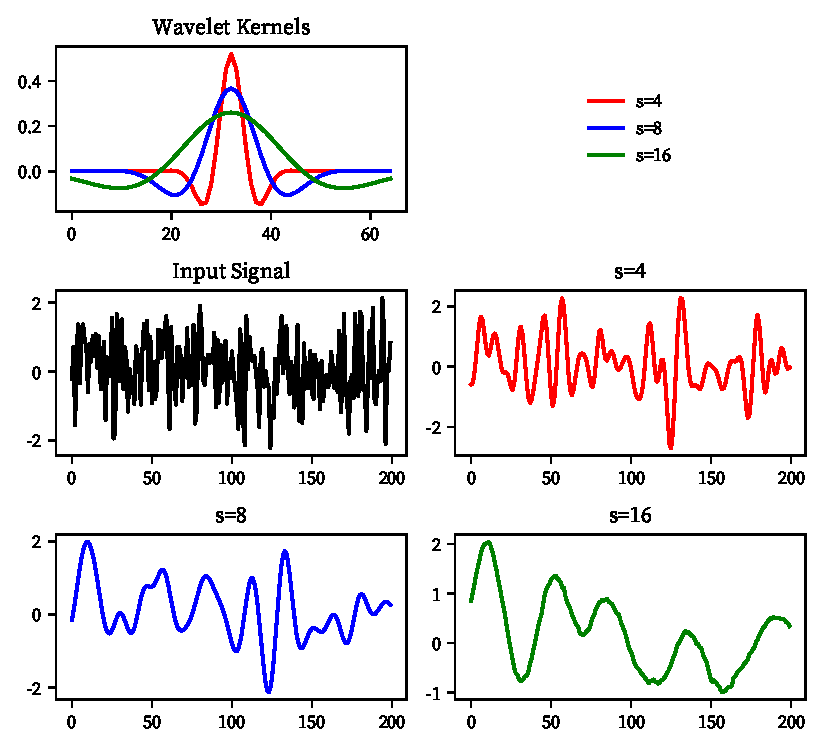
\includegraphics[width=\linewidth]{wavelet-transform.pdf}
    \caption{(Top) Normalized Morlet-style wavelet kernels at scales [4, 8, 16]. (Bottom) Input–output relationships: Gaussian white noise input (top–left) and its filtered components using the respective wavelets (red: $s=4$, blue: $s=8$, green: $s=16$). Responses exhibit progressive high–frequency suppression and temporal smoothing with increasing scale. The visualizer implements bank normalization and preserves temporal resolution via same–padding convolutions (using a $\beta$–spline differentiable implementation).}

    \label{fig:wavelet-transform}
\end{figure}

We optimize both signal-space and wavelet-domain reconstructions through:

\begin{equation}
    \mathcal{L} = \lambda_1 \|\mathbf{\hat{X}} - \mathbf{X}\|_2^2 + \lambda_2 \|\mathbf{\hat{X}}_{\text{wave}} - \mathbf{X}_{\text{wave}}\|_2^2
\end{equation}

where $\lambda_1=1$, $\lambda_2=0.5$ balance reconstruction error and wavelet transform loss.



\section{Experiments}

\subsection{Dataset Generation}
\label{sec:dataset}

The synthetic dataset is generated through a 48-hour MATLAB simulation sampling Ku-band (10.7-12.7 GHz) interference scenarios at 10-second intervals, producing 17,281 temporal snapshots following \cite{saifaldawlaGenAIBasedModelsNGSO2024}. Each instance contains synchronized time-domain and frequency-domain representations: an 800-point waveform captures signal amplitudes, while an 800-bin spectral magnitude is derived via FFT processing.

Binary classification labels are assigned through link budget analysis, where class 0 denotes non-interference scenarios ($\text{INR} < \Gamma_{\text{th}}$) below the system protection threshold, and class 1 indicates substantial interference ($\text{INR} \geq \Gamma_{\text{th}}$) exceeding operational limits. We normalize the input signals in both domains separately to zero mean and unit variance.

The dataset is partitioned under anomaly detection constraints, with training (11,509 samples) and validation (1,302 samples) sets containing exclusively non-interference data (class 0). The test set comprises balanced proportions of 2,235 class 0 and 2,235 class 1 instances. The simulation incorporates time-varying link losses with 0-9 dB range, extreme interference cases reaching peak aggregate INR of 32.47 dB, with background CNR fluctuations between 6.40-15.40 dB.

\subsection{Evaluation Results}

\begin{figure}[tb]
    \centering
    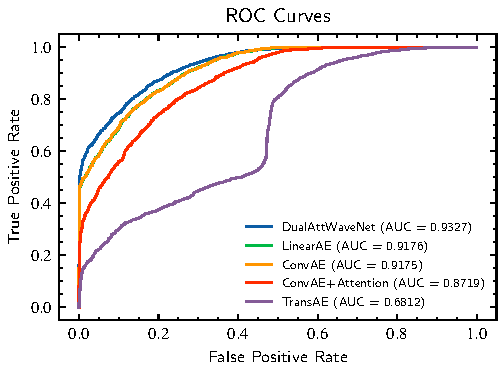
\includegraphics[width=0.8\linewidth]{roc-comparison.pdf}
    \caption{ROC curves for DualAttnWaveNet and baseline models. DualAttnWaveNet achieves the highest AUC score.}
    \label{fig:roc_comparison}
\end{figure}

DualAttWaveNet achieves state-of-the-art interference detection performance across metrics, as shown in Table~\ref{tab:main_results}. With an AUC of 0.9327, it outperforms ConvAE (0.9175), ConvAE+Attention (0.8719), and TransAE (0.6812), as quantified by ROC analysis (\figurename~\ref{fig:roc_comparison}). Notably, the model surpasses the previous best method, TrID \cite{saifaldawlaGenAIBasedModelsNGSO2024}, which achieved AUCs of 0.8318 (time domain) and 0.7106 (spectral domain), highlighting superior cross-modal harmonization through dual-attention synergy.

\begin{table}[t]
    \caption{Performance Comparison of DualAttnWaveNet Against Baseline Models}
    \label{tab:main_results}
    \centering
    \resizebox{\linewidth}{!}{\begin{tabular}{lcccc}
            \toprule
            \textbf{Model}  & \textbf{Accuracy (\%) } $\uparrow$ & \textbf{F1 Score} $\uparrow$ & \textbf{AUC}$\uparrow$ & \textbf{FLOPS (G)} \\
            \midrule
            DualAttnWaveNet & 0.8351                             & 0.8351                       & 0.9327                 & 5.19               \\
            \cmidrule{1-5}
            LinearAE        & 0.8149                             & 0.8149                       & 0.9176                 & 0.49               \\
            CNNAE           & 0.8170                             & 0.8169                       & 0.9175                 & 0.50               \\
            CNNAE+Attention & 0.7695                             & 0.7691                       & 0.8718                 & 3.01               \\
            TrID            & 0.8318                             & 0.8321                       & 0.8318                 & 50.00     \\
            Transformer AE  & 0.6812                             & 0.5921                       & 0.6812                 & 26.43              \\
            \bottomrule
        \end{tabular}}
\end{table}

\begin{table}[t]
    \caption{Ablation Study of DualAttnWaveNet Components}
    \label{tab:ablation}
    \centering
    \resizebox{\linewidth}{!}{
        \begin{tabular}{lccc}
            \toprule
            \textbf{Model Variant} & \textbf{Accuracy (\%)} $\uparrow$ & \textbf{F1 Score} $\uparrow$ & \textbf{AUC} $\uparrow$ \\
            \midrule
            DualAttnWaveNet (Full) & 0.8351                            & 0.8351                       & 0.9327                  \\
            \cmidrule{1-4}
            w/o Mutual Attention   & 0.8289                            & 0.8288                       & 0.9294                  \\
            w/o Wavelet Loss       & 0.8273                            & 0.8273                       & 0.9283                  \\
            Vanilla Implementation & 0.7995                            & 0.7975                       & 0.9175                  \\
            \bottomrule
        \end{tabular}

    }

\end{table}



% \begin{table*}[t]
%     \caption{Performance Comparison of DualAttnWaveNet Against Baseline Models}
%     \label{tab:main_results}
%     \centering
%     \begin{tabular}{lcccc}
%         \toprule
%         \textbf{Model}  & \textbf{Accuracy (\%) } $\uparrow$ & \textbf{F1 Score} $\uparrow$ & \textbf{AUC}$\uparrow$ & \textbf{FLOPS (G)}$\downarrow$ \\
%         \midrule
%         DualAttnWaveNet & 0.8351                             & 0.8351                       & 0.9327                 & 0.00                           \\
%         \cmidrule{1-5}
%         LinearAE        & 0.8149                             & 0.8149                       & 0.9176                 & 0.00                           \\
%         CNNAE           & 0.8170                             & 0.8169                       & 0.9175                 & 0.00                           \\
%         CNNAE+Attention & 0.7695                             & 0.7691                       & 0.8718                 & 0.00                           \\
%         TrID            & 0.8318                             & 0.8321                       & 0.8318                 & 0.00                           \\
%         Transformer AE  & 0.6812                             & 0.5921                       & 0.6812                 & 0.00                           \\
%         \bottomrule
%     \end{tabular}
% \end{table*}


For the confusion matrix analysis, the detection threshold was determined as the sum of the mean and standard deviation of the reconstruction error computed on the validation set  Reconstruction error over this threshold is considered to be in class 1. \figurename~\ref{fig:confusion_matrix} shows that DualAttWaveNet has balanced precision-recall tradeoff (F1: 83.51\%). Baselines exhibit critical limitations: ConvAE+Attention suffers a 4.56\% AUC drop relative to ConvAE, shows  the insufficiency of naive attention for cross-domain alignment. TransAE’s poor convergence (AUC: 0.6812) suggests transformer architectures is hard to converge to optimal point during training.


\begin{figure}[tb]
    \centering
    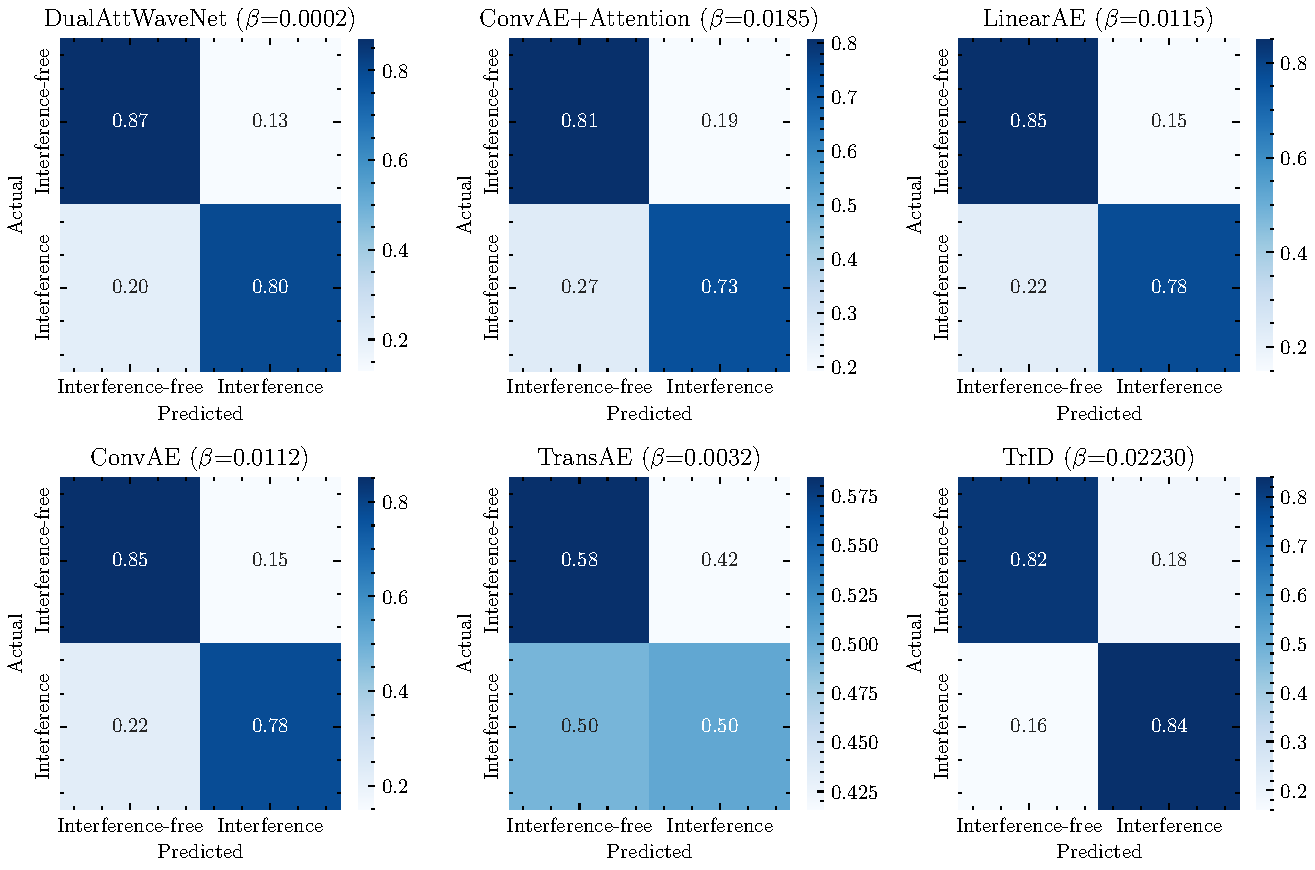
\includegraphics[width=\linewidth]{confusion.pdf}
    \caption{Confusion matrix for DualAttnWaveNet and baselines on the test set}
    \label{fig:confusion_matrix}
\end{figure}

DualAttnWaveNet processes 5,000 batched samples (batch size: 128, 800 timesteps/sample) in under one second. While its FLOPs (5.19G) exceed those of lighter models (Table \ref{tab:main_results}), it significantly outperforms TrID (50.00G) and Transformer AE (26.43G) in computational efficiency. This is due it only uses one dot-product attention, instead of multi-head attention implemented in TrID and TransAE. 


\subsection{Ablation Study}

To validate the architectural design of DualAttWaveNet, systematic component ablation experiments were conducted (Table \ref{tab:ablation}). The full configuration achieves peak performance, while removing the mutual attention module reduces AUC to 0.9294 (−0.33\%), demonstrating its necessity for temporal-spectral feature alignment. Further ablation of the wavelet coherence loss degrades performance to 0.9283 AUC (−0.44\% from full model), confirming the loss’s role in preserving time-frequency structure. The baseline implementation (no mutual attention or wavelet loss) yields the lowest metrics (AUC: 0.9175, Accuracy: 79.95\%), underperforming all proposed variants.

% \begin{table*}[t]
%     \caption{Ablation Study of DualAttnWaveNet Components}
%     \label{tab:ablation}
%     \centering
%     \begin{tabular}{lccc}
%         \toprule
%         \textbf{Model Variant} & \textbf{Accuracy (\%)} $\uparrow$ & \textbf{F1 Score} $\uparrow$ & \textbf{AUC} $\uparrow$ \\
%         \midrule
%         DualAttnWaveNet (Full) & 0.8367                            & 0.8366                       & 0.9327                  \\
%         \cmidrule{1-4}
%         w/o Mutual Attention   & 0.8289                            & 0.8288                       & 0.9294                  \\
%         w/o Wavelet Loss       & 0.8273                            & 0.8273                       & 0.9283                  \\
%         Vanilla Implementation & 0.7995                            & 0.7975                       & 0.9175                  \\
%         \bottomrule
%     \end{tabular}
%     \vspace{2pt}

% \end{table*}

\section{Conclusion}

In this paper, we have presented DualAttWaveNet, a multimodal interference detection framework designed for GSO/LEO coexistence scenarios. The model fuses time-domain waveforms and spectral representations via a bidirectional attention mechanism, enabling cross-domain feature alignment with reduced computational overhead (5.19 GFLOPs). Through multi-scale wavelet regularization, reconstruction error is enforced across temporal and spectral resolutions. Evaluation under synthesized Ku-band interference scenarios demonstrated improved AUC (0.9327) and accuracy (83.51\%) relative to SOTA baseline. The model processed 5,000 test samples with an average latency of 97.2 ms per sample on a single NVIDIA 3050Ti GPU. Future work will evaluate model on different overlap scenarios and explore other wavelet families for regularization.

\bibliographystyle{IEEEtran}
\bibliography{references}

\end{document}
